\documentclass[11pt]{article}

\newcommand{\yourname}{}
\newcommand{\yourcollaborators}{}

\def\comments{0}

%format and packages%\usepackage{algorithm, algorithmic}
\usepackage{algpseudocode}
\usepackage{amsmath, amssymb, amsthm}
\usepackage{enumerate}
\usepackage{enumitem}
\usepackage{framed}
\usepackage{verbatim}
\usepackage[margin=1.0in]{geometry}
\usepackage{multirow}

\usepackage{microtype}


\usepackage{graphicx}
\usepackage{tikz}
\usetikzlibrary{automata, positioning, arrows.meta}

	\definecolor{processblue}{cmyk}{0.96,0,0,0}


\usepackage{kpfonts}
\usepackage{palatino}
	\DeclareMathAlphabet{\mathtt}{OT1}{cmtt}{m}{n}
	\SetMathAlphabet{\mathtt}{bold}{OT1}{cmtt}{bx}{n}
	\DeclareMathAlphabet{\mathsf}{OT1}{cmss}{m}{n}
	\SetMathAlphabet{\mathsf}{bold}{OT1}{cmss}{bx}{n}
	\renewcommand*\ttdefault{cmtt}
	\renewcommand*\sfdefault{cmss}
	\renewcommand{\baselinestretch}{1.06}
\usepackage{tikz}
	\usetikzlibrary{positioning}
	\definecolor{processblue}{cmyk}{0.96,0,0,0}
    \usetikzlibrary{matrix,arrows}

\tikzset{
->, % makes the edges directed
>=Stealth, % makes the arrow heads bold
node distance=3cm, % specifies the minimum distance between two nodes. Change if necessary.
every state/.style={thick, fill=gray!10}, % sets the properties for each ’state’ node
initial text=$ $, % sets the text that appears on the start arrow
}
	
\usepackage{hyperref}

\hypersetup{
	linktocpage=true,
	colorlinks=true,				% false: boxed links; true: colored links
	linkcolor=blue,		% color of internal links
	citecolor=blue,	% color of links to bibliography
	urlcolor=blue,		% color of external links
}

\usepackage[boxruled,vlined,nofillcomment]{algorithm2e}
	\SetKwProg{Fn}{Function}{\string:}{}
	\SetKwFor{While}{While}{}{}
	\SetKwFor{For}{For}{}{}
	\SetKwIF{If}{ElseIf}{Else}{If}{:}{ElseIf}{Else}{:}
	\SetKw{Return}{Return}

%enclosure macros
\newcommand{\paren}[1]{\ensuremath{\left( {#1} \right)}}
\newcommand{\bracket}[1]{\ensuremath{\left\{ {#1} \right\}}}
\renewcommand{\sb}[1]{\ensuremath{\left[ {#1} \right\]}}
\newcommand{\ab}[1]{\ensuremath{\left\langle {#1} \right\rangle}}

%probability macros
\newcommand{\ex}[2]{{\ifx&#1& \mathbb{E} \else \underset{#1}{\mathbb{E}} \fi \left[#2\right]}}
\newcommand{\pr}[2]{{\ifx&#1& \mathbb{P} \else \underset{#1}{\mathbb{P}} \fi \left[#2\right]}}
\newcommand{\var}[2]{{\ifx&#1& \mathrm{Var} \else \underset{#1}{\mathrm{Var}} \fi \left[#2\right]}}

%useful CS macros
\newcommand{\poly}{\mathrm{poly}}
\newcommand{\polylog}{\mathrm{polylog}}
\newcommand{\zo}{\{0,1\}}
\newcommand{\pmo}{\{\pm1\}}
\newcommand{\getsr}{\gets_{\mbox{\tiny R}}}
\newcommand{\card}[1]{\left| #1 \right|}
\newcommand{\set}[1]{\left\{#1\right\}}
\newcommand{\negl}{\mathrm{negl}}
\newcommand{\eps}{\varepsilon}
\DeclareMathOperator*{\argmin}{arg\,min}
\DeclareMathOperator*{\argmax}{arg\,max}
\newcommand{\eqand}{\qquad \textrm{and} \qquad}
\newcommand{\ind}[1]{\mathbb{I}\{#1\}}
\newcommand{\sslash}{\ensuremath{\mathbin{/\mkern-3mu/}}}

%mathbb
\newcommand{\N}{\mathbb{N}}
\newcommand{\R}{\mathbb{R}}
\newcommand{\Z}{\mathbb{Z}}
%mathcal
\newcommand{\cA}{\mathcal{A}}
\newcommand{\cB}{\mathcal{B}}
\newcommand{\cC}{\mathcal{C}}
\newcommand{\cD}{\mathcal{D}}
\newcommand{\cE}{\mathcal{E}}
\newcommand{\cF}{\mathcal{F}}
\newcommand{\cL}{\mathcal{L}}
\newcommand{\cM}{\mathcal{M}}
\newcommand{\cO}{\mathcal{O}}
\newcommand{\cP}{\mathcal{P}}
\newcommand{\cQ}{\mathcal{Q}}
\newcommand{\cR}{\mathcal{R}}
\newcommand{\cS}{\mathcal{S}}
\newcommand{\cU}{\mathcal{U}}
\newcommand{\cV}{\mathcal{V}}
\newcommand{\cW}{\mathcal{W}}
\newcommand{\cX}{\mathcal{X}}
\newcommand{\cY}{\mathcal{Y}}
\newcommand{\cZ}{\mathcal{Z}}

\newcommand{\opt}{\textsc{opt}}

%theorem macros
\newtheorem{thm}{Theorem}
\newtheorem{lem}[thm]{Lemma}
\newtheorem{fact}[thm]{Fact}
\newtheorem{clm}[thm]{Claim}
\newtheorem{rem}[thm]{Remark}
\newtheorem{coro}[thm]{Corollary}
\newtheorem{prop}[thm]{Proposition}
\newtheorem{conj}[thm]{Conjecture}

\theoremstyle{definition}
\newtheorem{defn}[thm]{Definition}


\newcommand{\instructor}{Drew van der Poel}
\newcommand{\hwnum}{2}
\newcommand{\hwdue}{Friday, July 22 at 11:59pm via \href{https://www.gradescope.com/courses/406943}{Gradescope}}

\theoremstyle{theorem}
\newtheorem{prob}{Problem}
\newtheorem{sol}{Solution}

\definecolor{cit}{rgb}{0.05,0.2,0.45} 
\newcommand{\solution}{\medskip\noindent{\color{blue}\textbf{Solution:}}}

\begin{document}
{\Large 
\begin{center}{CS3800: Theory of Computation} --- Summer II '22 --- \instructor \end{center}}
{\large
\vspace{10pt}
\noindent Homework~\hwnum \vspace{2pt}\\
Due~\hwdue}

\bigskip
{\large
\noindent Name: Steve Liu  \yourname \vspace{2pt}\\ Collaborators: Ares Do, Jamie Lin, Eric Chapelaine, Michael Fang, HwiJoon Lee, Jaron Cui \yourcollaborators}

\vspace{15pt}
\begin{itemize}

\item Make sure to put your name on the first page.  If you are using the \LaTeX~template we provided, then you can make sure it appears by filling in the \texttt{yourname} command.

\item This assignment is due~\hwdue.  No late assignments will be accepted.  Make sure to submit something before the deadline.

\item Solutions must be typeset.  If you need to draw any diagrams, you may draw them by hand as long as they are embedded in the PDF.  I recommend using the source file for this assignment to get started.

\item I encourage you to work with your classmates on the homework problems. \emph{If you do collaborate, you must write all solutions by yourself, in your own words.}  Do not submit anything you cannot explain.  Please list all your collaborators in your solution for each problem by filling in the \texttt{yourcollaborators} command.

\item Finding solutions to homework problems on the web, or by asking students not enrolled in the class is strictly forbidden.

\end{itemize}





\newpage

\begin{prob} Converting NFAs to DFAs (\emph{6 points})\end{prob}


Convert the following NFA to a DFA. Your DFA should be as simple as possible (e.g. any states which cannot be reached from the initial state should be removed). Note $\Sigma = \{0,1,2\}$.

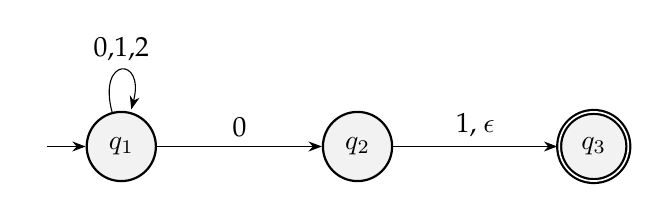
\begin{tikzpicture}
\node[state, initial] (q1) {$q_1$};
\node[state, right of=q1] (q2) {$q_2$};
\node[state, accepting, right of=q2] (q3) {$q_3$};
\draw (q1) edge[above] node{0} (q2)
(q1) edge[loop above] node{0,1,2} (q1)
(q2) edge[above] node{1, $\epsilon$} (q3);

\end{tikzpicture}

\solution
\\WORK FOR PROBLEM ON NEXT PAGE 
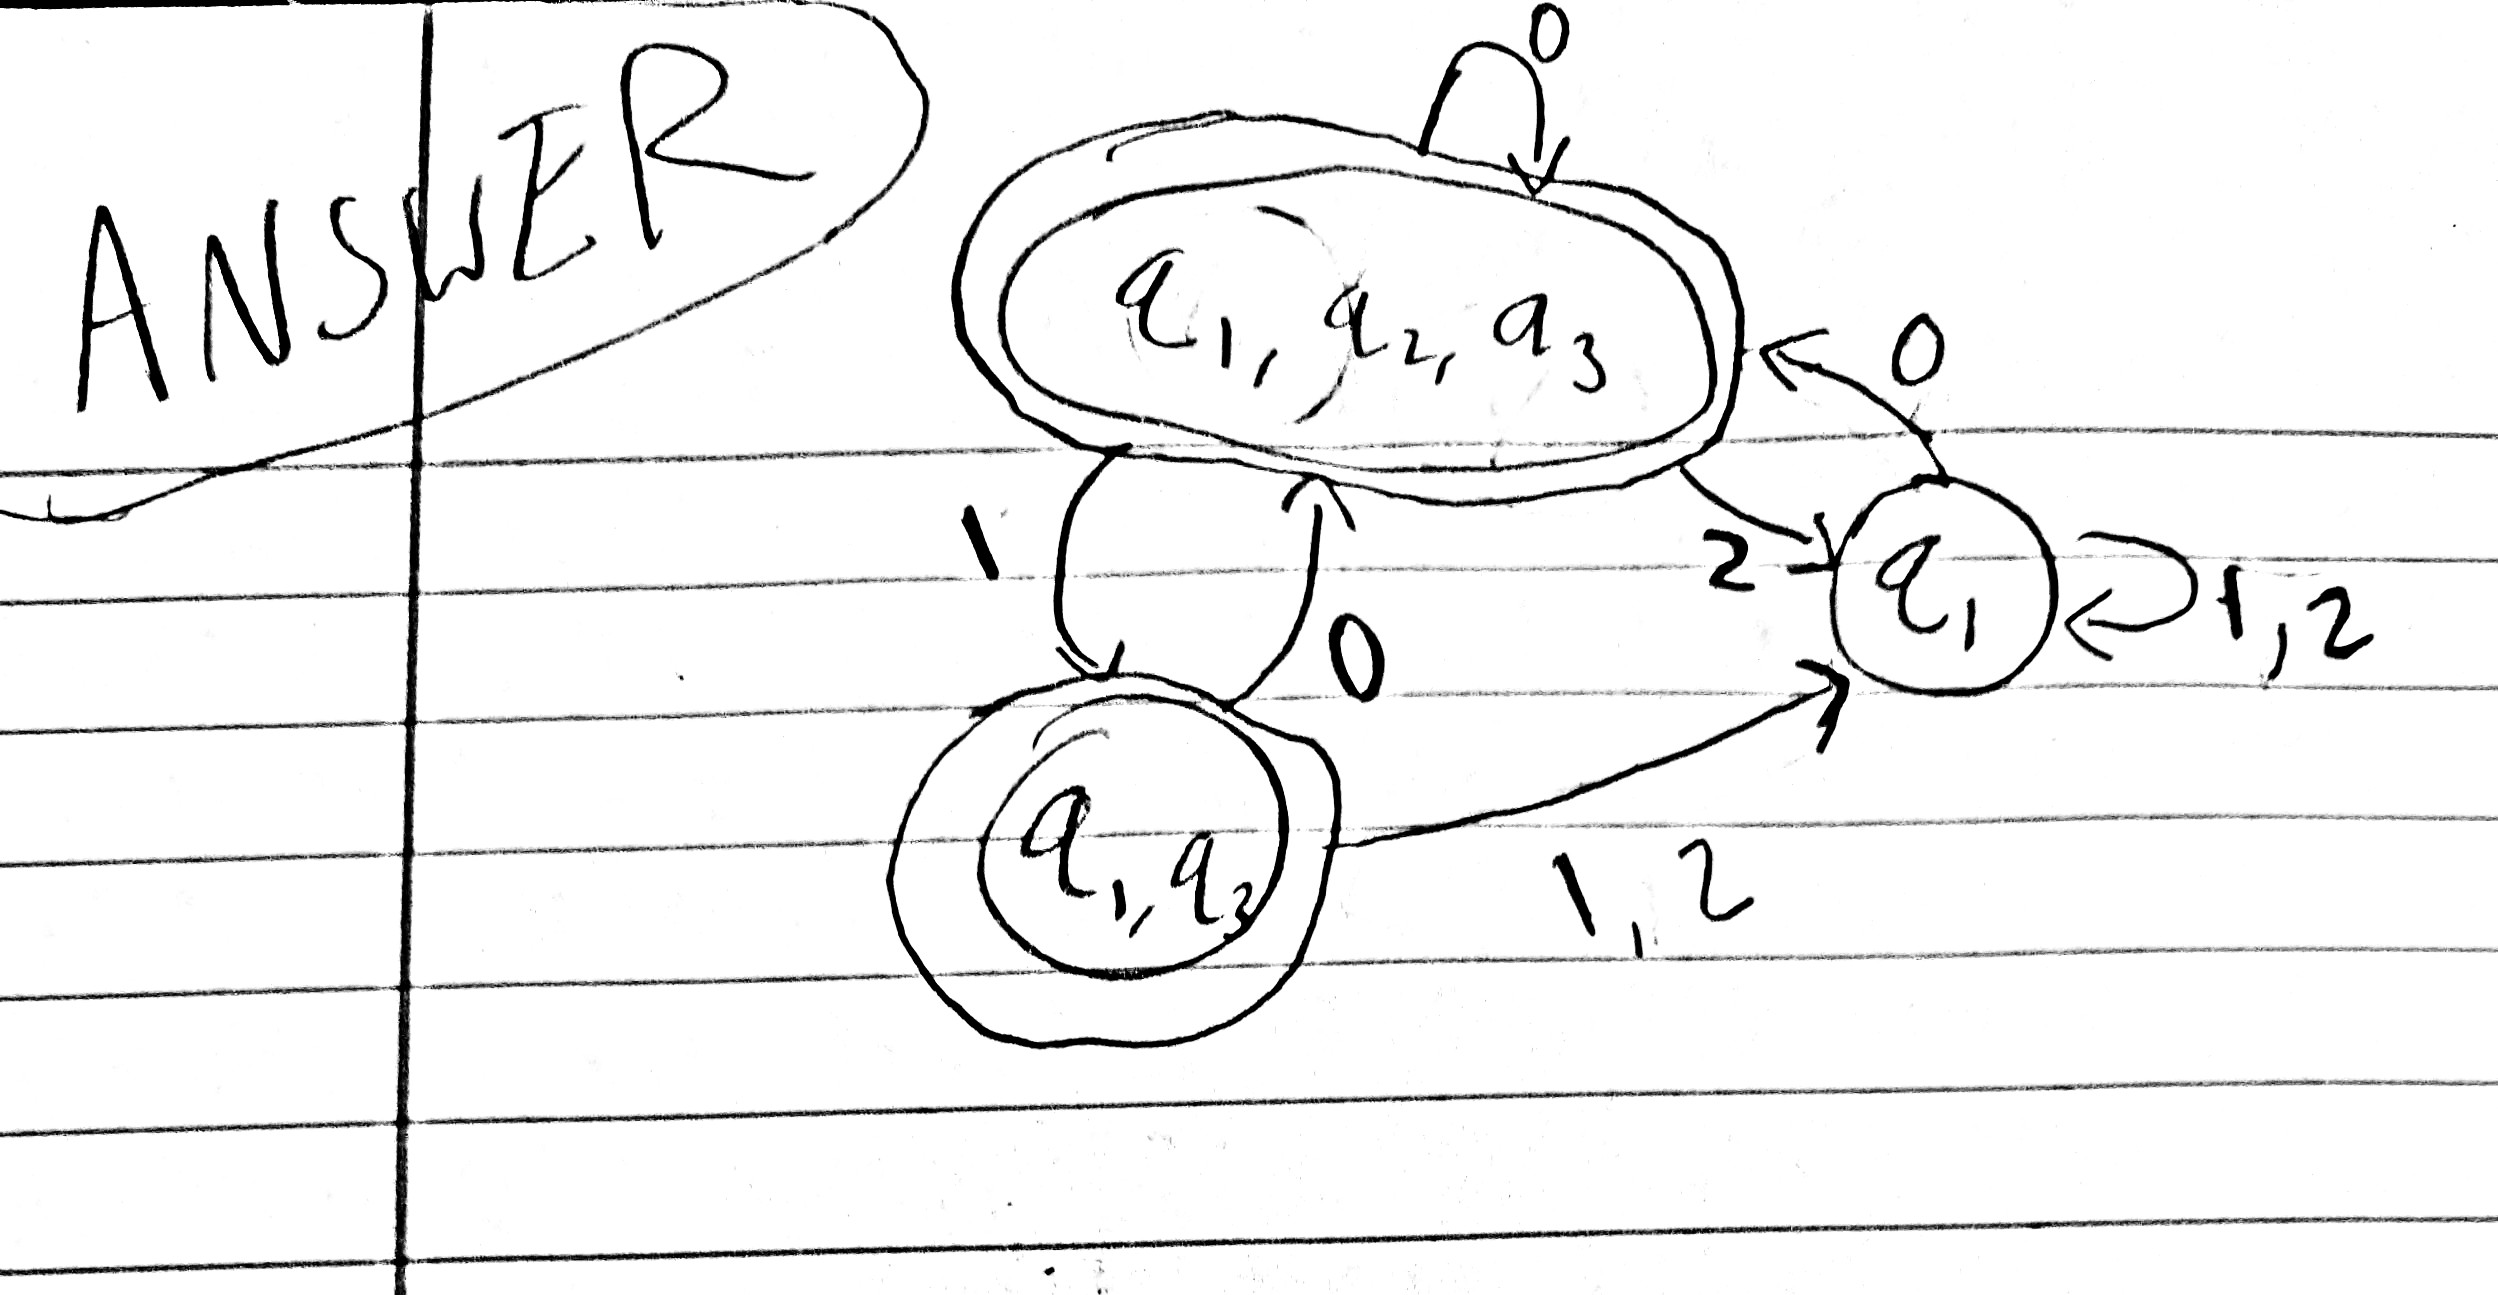
\includegraphics[angle=-90,origin=c, scale=0.11, width= 12cm]{./p1_images/ans.jpg}

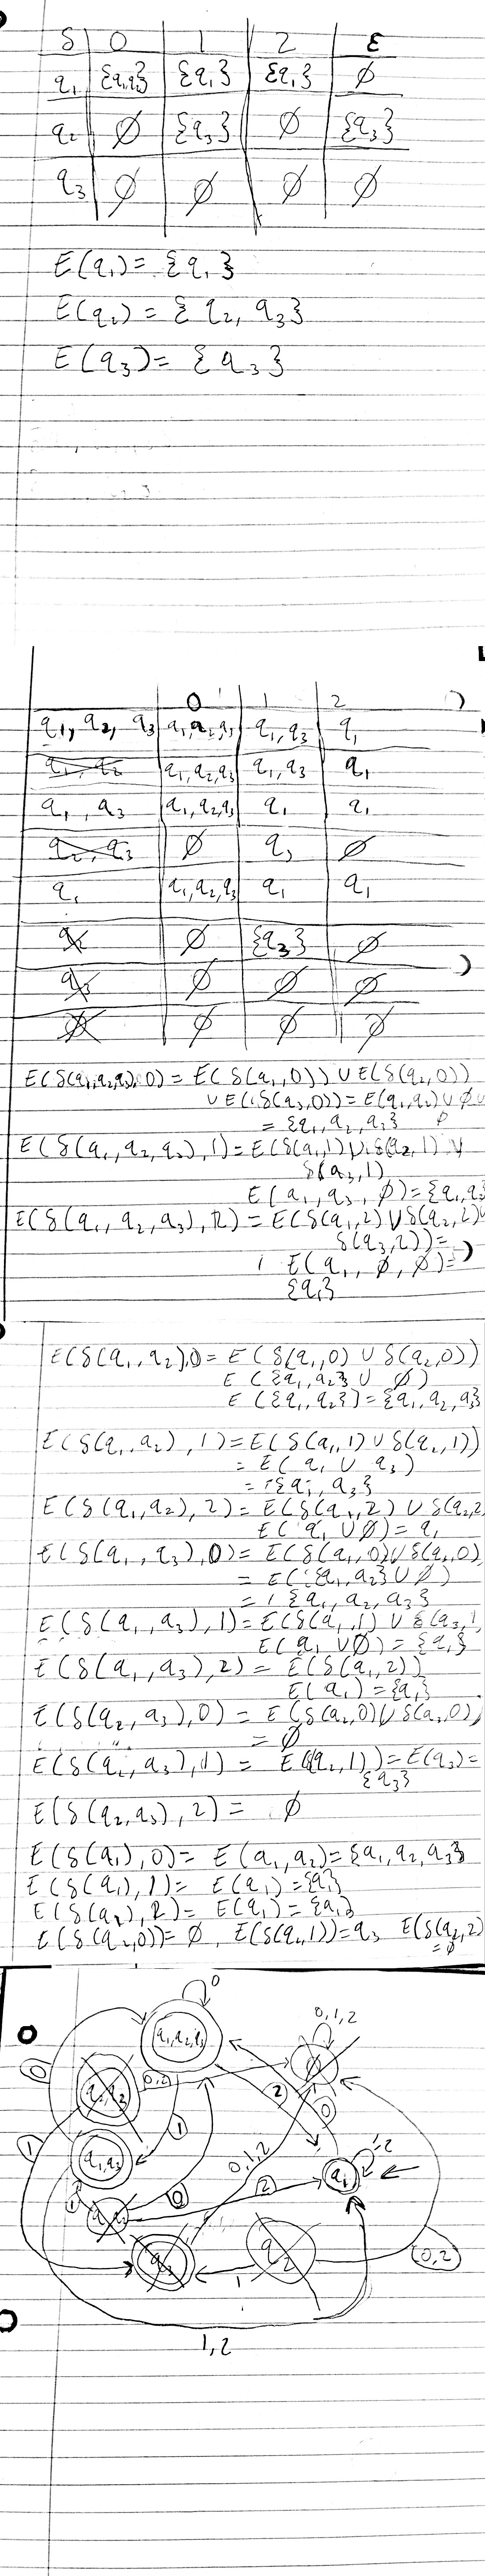
\includegraphics[scale=0.1]{./p1_images/work.jpg}




\newpage

\begin{prob} Regular Expressions (\emph{6 points})\end{prob}

Give a regular expression for the language of words over $\Sigma = \{0, 1\}$ which have an equal number of copies of 01 and 10 as substrings (note: these copies need not be disjoint). Show why your regular expression accepts the words $10101$, $0101110$, $111$, and $111111011$. Explain why it does not generate $0101$. Provide brief justification for why your regular expression works as desired.

\solution

\noindent REGULAR EXPRESSION: 0(0 $\cup$ 1)*0 $\cup$ 1(0 $\cup$ 1)*1 $\cup$ $ \epsilon $ $\cup$ 1 $\cup$ 0 \\

\noindent 10101 $\rightarrow$ 1(010)1 is in 1(0 $\cup$ 1)*1 $\rightarrow$ you have the left and right side 1's with 010 in the middle which is in (0 $\cup$ 1)* \\~\\
\noindent 0101110 $\rightarrow$ 0(10111)0 is in 0(0 $\cup$ 1)*0  $\rightarrow$ you have the left and right side 0's with 10111 in the middle which is in (0 $\cup$ 1)* \\~\\
\noindent 111 $\rightarrow$ 1(1)1 is in 1(0 $\cup$ 1)*1  $\rightarrow$ you have the left and right side 1's with 1 in the middle which is in (0 $\cup$ 1)* \\~\\
\noindent 111111011 $\rightarrow$ 1(1111101)1 is in 1(0 $\cup$ 1)*1  $\rightarrow$ you have the left and right side 1's with 1111101 in the middle which is in (0 $\cup$ 1)* \\~\\
\noindent 0101 cannot be generated because it does not belong in 0(0 $\cup$ 1)*0 as it does not start or end in 0, nor 1(0 $\cup$ 1)*1 for the same reason (it does not start or end with 1), nor is it an empty string, nor the string 1, and it is not the string 0.   \\~\\

\noindent EXPLANATION: Getting the easiest cases out of the way, this language should accept the empty string, 1, and 0 since they all have zero 01s and 10s.
\noindent For other strings, we can break down the possibilities into two separate cases: \\ ~ \\

\noindent Case 1: The string begins with a 1, the next input in the string can either be a 0 or a 1. We can disregard all 1's until the first 0 since the number of 01's and 10's do not change. Once we reach our first 0, then we get to a case where there are one 10's and zero 01's in the string. Turns out, because of the "non-disjoint" rule of this language, if we let $n$ be the length of the string, the number of 10's can be counted in the first $n-1$ substring and the number of 01 can be counted in the last $n-1$ substring (i.e. take the string, 10101 has 2 01's and 2 10's, the first $n-1$th substring = 1010 has 2 10's and last $n-1th$ substring = 0101 has 2 01's). 
As a result of this rule, the number of 10's will always be exactly one greater than the number of 01's if the string starts with a 1 and ends in a 0 because the first 0 will always be able to create a 10 but the last 0 will never be able to create a matching 01.  
In order to guarantee that the first and last zeroes create an equivalent number 10's and 01's, the last input of the string has to be a 1 in order to match the last 0 in the string. \\~\\

\noindent Case 2: The string begins with a 0. This case is entirely symmetrical to the first case with the same idea but this time the number of 01's will always be exactly one greater than the number 10's if the string begins with 0 and ends in 1 for the same symmetrical reason mentioned in Case 1. To remediate this issue, we can basically do the same thing by enforcing that the last input of the string has to be a 0.
\newpage

\begin{prob} NFA to RegEx (\emph{9 points})\end{prob}

Consider the following NFAs. For each, convert it to a regular expression. Show all intermediate steps when building and simplifying the GNFA. You can omit transitions labeled with $\emptyset$.

$D_1$:

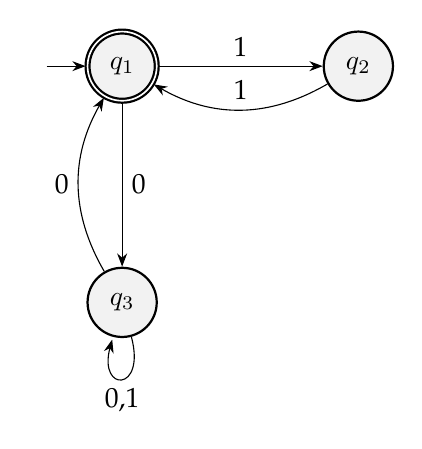
\begin{tikzpicture}
\node[state, accepting, initial] (q1) {$q_1$};
\node[state,  right of=q1] (q2) {$q_2$};
\node[state, below of=q1] (q3) {$q_3$};
\draw (q1) edge[above] node{1} (q2)
 (q1) edge[right] node{0} (q3)
 (q2) edge[bend left, above] node{1} (q1)
 (q3) edge[bend left, left] node{0} (q1)
(q3) edge[loop below] node{0,1} (q3);


\end{tikzpicture}\\

$D_2$:

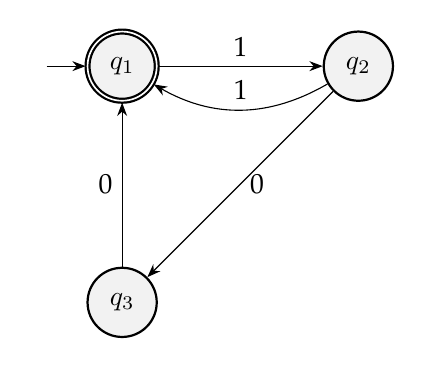
\begin{tikzpicture}
\node[state, accepting, initial] (q1) {$q_1$};
\node[state,  right of=q1] (q2) {$q_2$};
\node[state, below of=q1] (q3) {$q_3$};
\draw (q1) edge[above] node{1} (q2)
 (q2) edge[right] node{0} (q3)
 (q2) edge[bend left, above] node{1} (q1)
 (q3) edge[left] node{0} (q1);

\end{tikzpicture}



\solution \\
\noindent D1: $(11 \cup 0(0 \cup 1)$*$0)$*  \\ D2: $(11\cup100)$* \\ 1st image is D1, 2nd image is D2

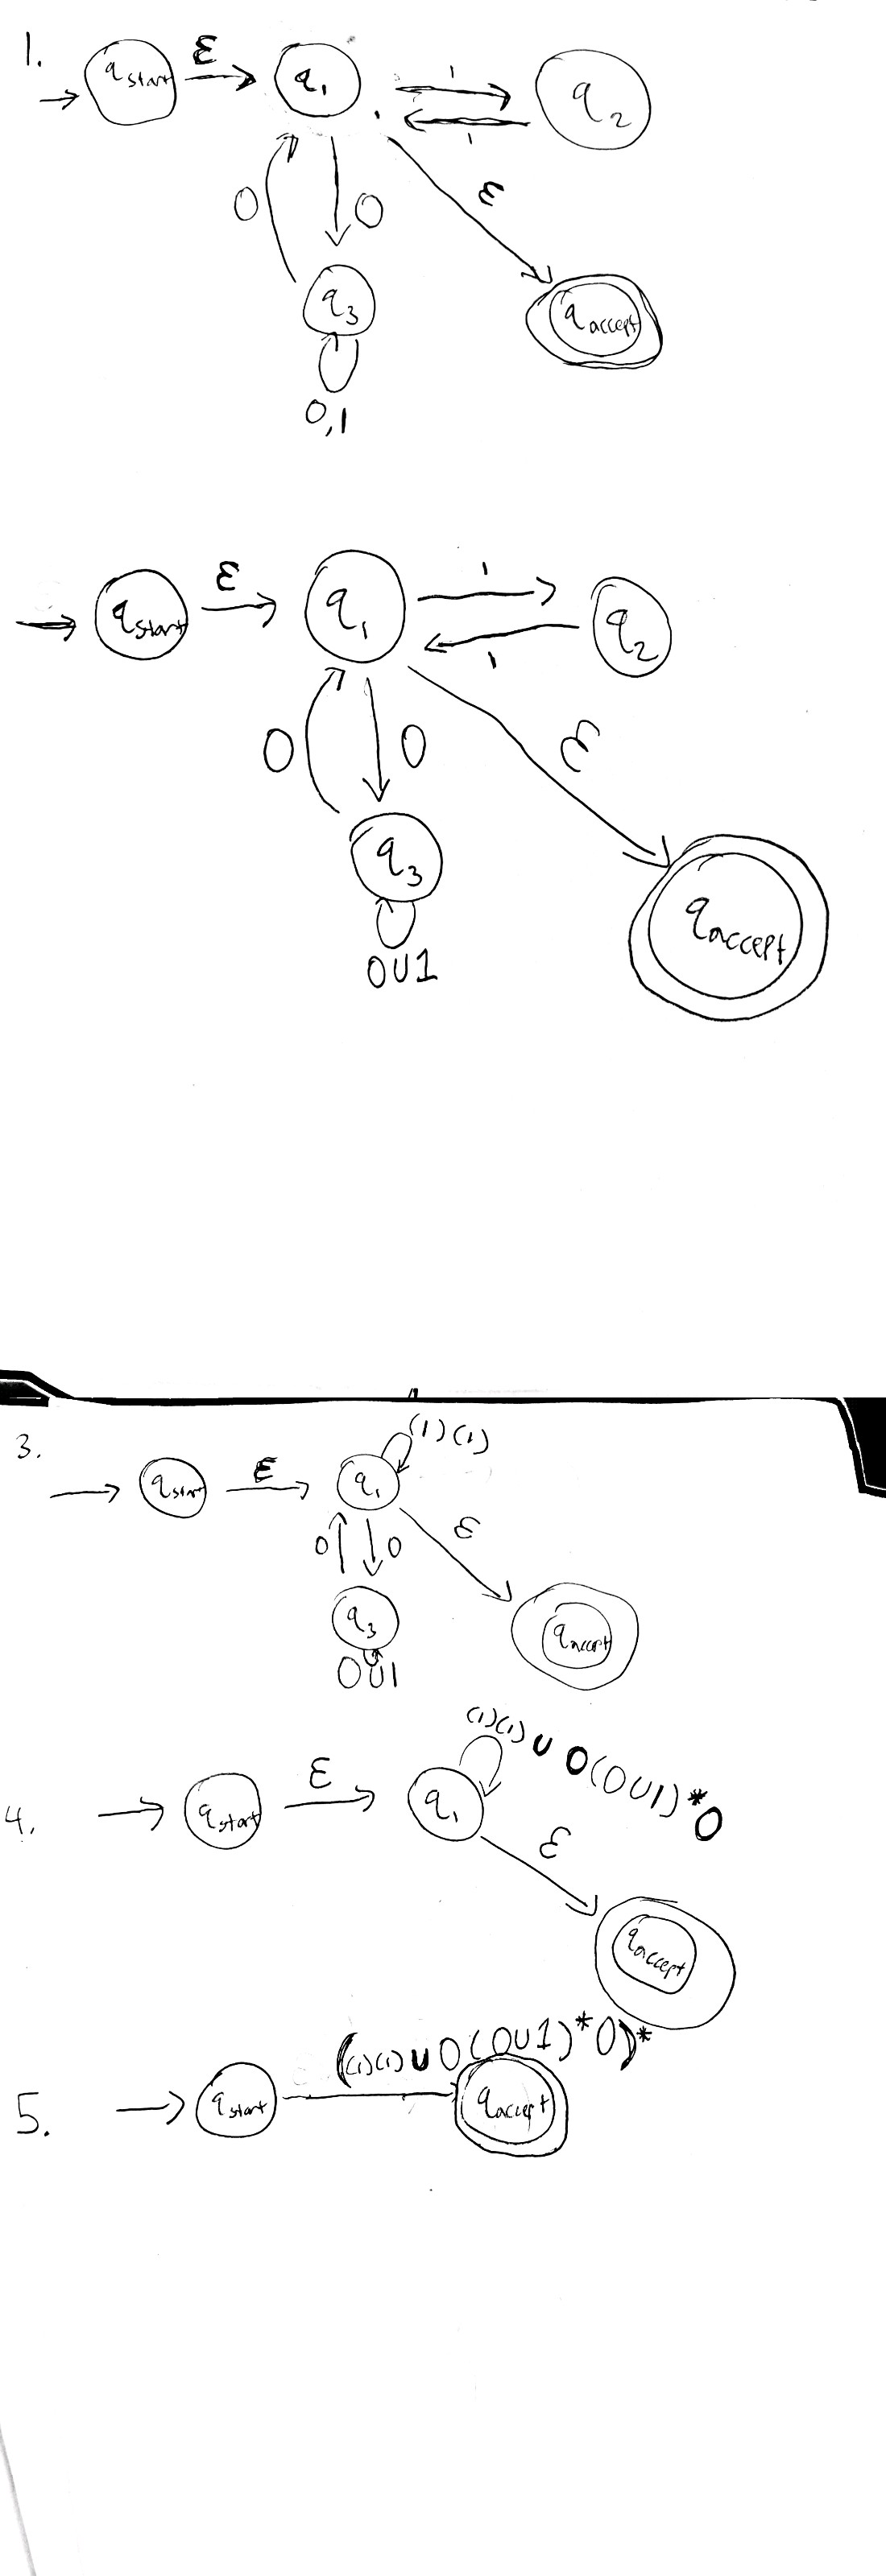
\includegraphics[width=10cm, height=28cm]{./p3_images/d1a.jpg} \\
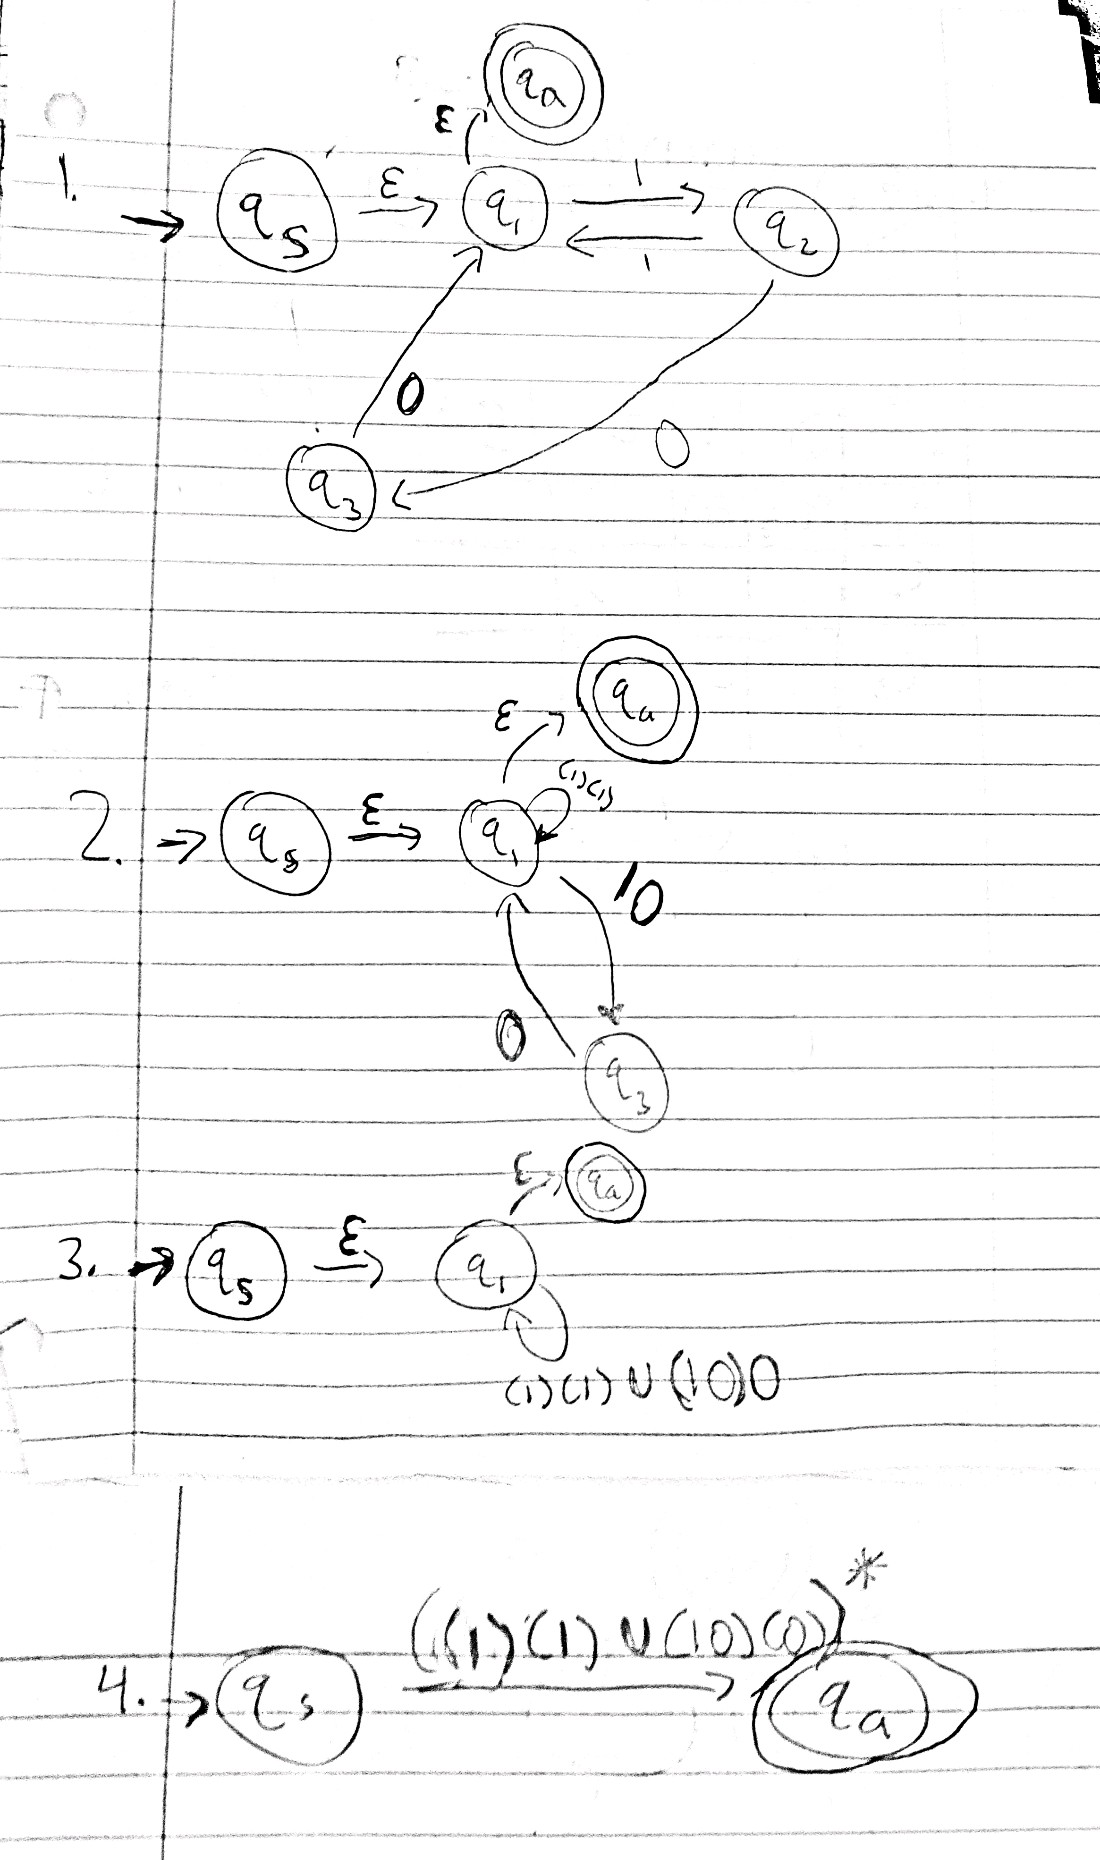
\includegraphics[width=15cm, height=25cm]{./p3_images/d2a.jpg}


\newpage

\begin{prob} Non-Regular Languages (\emph{9 points})\end{prob}

For each of the following languages over $\Sigma = \{g, q\}$, state whether or not it is regular. If it is, give a regular expression that describes it. If not, prove why using the Pumping Lemma. Note that we assume $\mathbb{N}$ (the natural numbers) to be the non-negative integers ($\{0, 1, 2, \dots\}$).

\begin{enumerate}[label=(\alph*)]



\item \textbf{[3 pts.]}  $L_1 = \{w |  w\in \{0,1\}^*; \text{number of 00 substrings is the same as the number of 11 substrings}\}$

\solution 
\\ Assume true, that $L_1$ is a regular language so the Pumping Lemma applies to $L_1$. Let $P$ be the pumping length. Let $S = (00)^P(11)^P$. We know that via the Pumping Lemma, $\left\lvert xy \right\rvert \leq P$
which means that $y$ must consist of some number of pairs of only zeroes for string $S$. We also know that the Pumping Lemma states $xy^iz \subseteq L_1$ which is not true when $i = 3$ for $S$ since $xyyyz \nsubseteq L_1$ as we will add more 00's to the string resulting in it having more 00's than we will have 11's. Thus, by contradiction, $L_1$ does not uphold the Pumping Lemma which means that $L_1$ is not regular.

\item \textbf{[3 pts.]}  $L_2 = \{0^n1^m | n,m \geq 5; n,m \in \mathbb{N}\}$

\solution 
\\ There has to be atleast five 0's in the string and five 1's in the string where all of the zeroes must be before all of the ones. Thus the regular expression for this language would be:
(00000)(0)*(11111)(1)*

\item \textbf{[3 pts.]}  $L_3 = \{w |  w\in \{0,1\}^*; \text{the length of w is odd and contains a 1 as the middle character}\}$

\solution 
\\ Assume true, that $L_3$ is a regular language so the Pumping Lemma applies to $L_3$. Let $P$ be the pumping length. Let $S = (00)^P1(00)^P$. We know that via the Pumping Lemma, $\left\lvert xy \right\rvert \leq P$, which means that $y$ must consist of some number of pairs of only zeroes for string $S$. However, we also know that the Pumping Lemma states $xy^iz \subseteq L_3$ which is not true when $i = 3$ for $S$ since adding any extra zeroes on the left side of $S$ will result in the left side having more 0s than the right side which means that the string no longer has a 1 in the middle. Thus, by contradiction, $L_3$ does not uphold the Pumping Lemma which means that $L_3$ is not regular.

\end{enumerate}





\end{document}
